\section{The Demo System Core}
\ToDo{
OLD text. 
Centralized webservice.
The list of datatypes used (images, audio, video, 3D pointclouds, 3D meshes) and how to identify them. The "no type" format for demos which have their own non-standard format.}

In this section we explain the demo system core, that is the responsible of the coordination of the other modules. One of its main issues is controlling the execution of the different experiments. Figure \ref{fig:core_diagram} shows a diagram that explains the modules and the messages passed when executing an experiment.

The core performs very simple actions like creating the directories, copy the blobs for the experiment, etc, for ensuring that everything is ready for a demo execution. It delegates in the Demo Dispatcher module (see Sec. \ref{sec:DemoDispatcher}) the selection of the computer for the experiment.

In order to distribute the load in several machines, this module checks the work load of each known DemoRunner modules (see Sect.~\ref{sec:DemoRunner}) and starts an algorithm demo execution on the less loaded machine. It uses a FIFO queue as a ``buffer'' to wait for a computer free to execute the demo and encapsulates an object to establishes the balancing policy that decides whether a process can leave the queue or not. Finally, the core uses the selected machine and waits until the experiment is finished. When it is finished, the core send to the archive module (see Sect.~\ref{sec:archive}) a JSON message for storing the experiment information.


\begin{figure}[!ht]
\centering
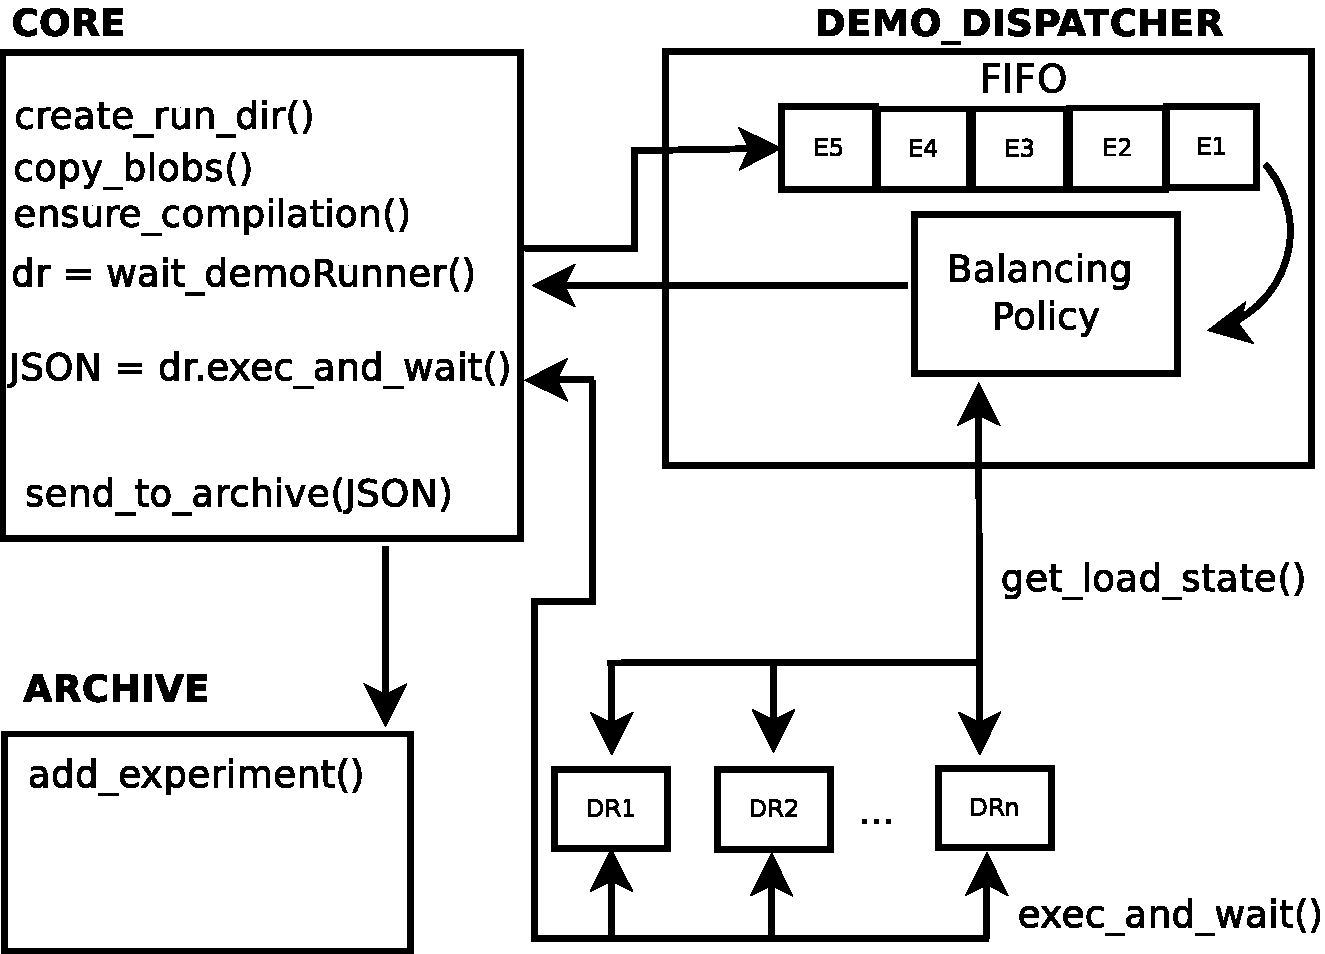
\includegraphics[width=0.7\columnwidth]{core/images/core_diagram.pdf}
\caption{Representation of the IPOL demos execution system.} 
\label{fig:core_diagram}
\end{figure}


\ToDo{Document it!}
